\Chapter{Az alkalmazás tervei}

\Section{Képernyő szerkezet}
Kezdetben összeállítottam egy tervet, arra, hogy nagyvonalakban hogyan is képzelem el a játék felületének felépítését, kinézetét. Ezen a kezdetleges rajzon elhelyeztem a kártyapaklikat, a kártyákat az azokon szereplő értékekkel, a zsetonokat és egy zsetongyűjtő panelt is. Az alapvető elképzeléseim az alapján születtek meg, hogy az alapjáték felépítése mind a fizikális, mind a digitális verzióban ehhez hasonlóan épül fel.

\begin{figure}[h]
\centering
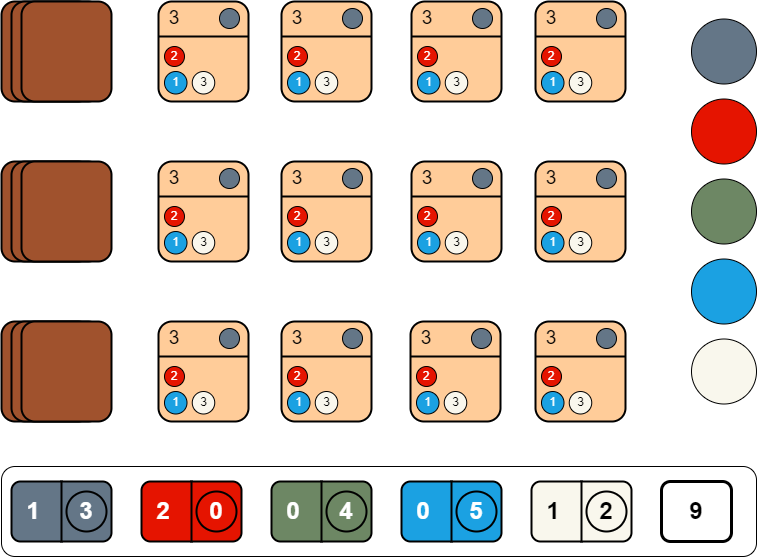
\includegraphics[scale=0.37]{images/screen_structure_plan.png}
\caption{A játék kezdetleges kinézeti terve.}
\label{fig:screen_structure_plan}
\end{figure}

\newpage

Az idő előrehaladtával formáltam mind a felépítést, mind a kinézetet, de a koncepció alapja megmaradt. A játék kapott egy hozzá illő hátteret, a kártyalapok színét is élőbbé tettem, a zsetonokat a halomban lévő számuk alapján megszámoztam és a zsetongyűjtő panelt is újraterveztem. Létrehoztam egy második panelt is a képernyő felső részén annak érdekében, hogy az adott játékos tudja követni az ellenfél részeredményeit is.
Emellett a jobb felső sarokba elhelyeztem egy új játék és egy játékszabályok feliratú gombot, a hozzájuk tartozó funciók ellátásához. Végezetül pedig megjelöltem a soron lévő játékost a hozzá tartozó panelének körberajzolásával és a játékost jellemző ikonnal.

\begin{figure}[h]
\centering
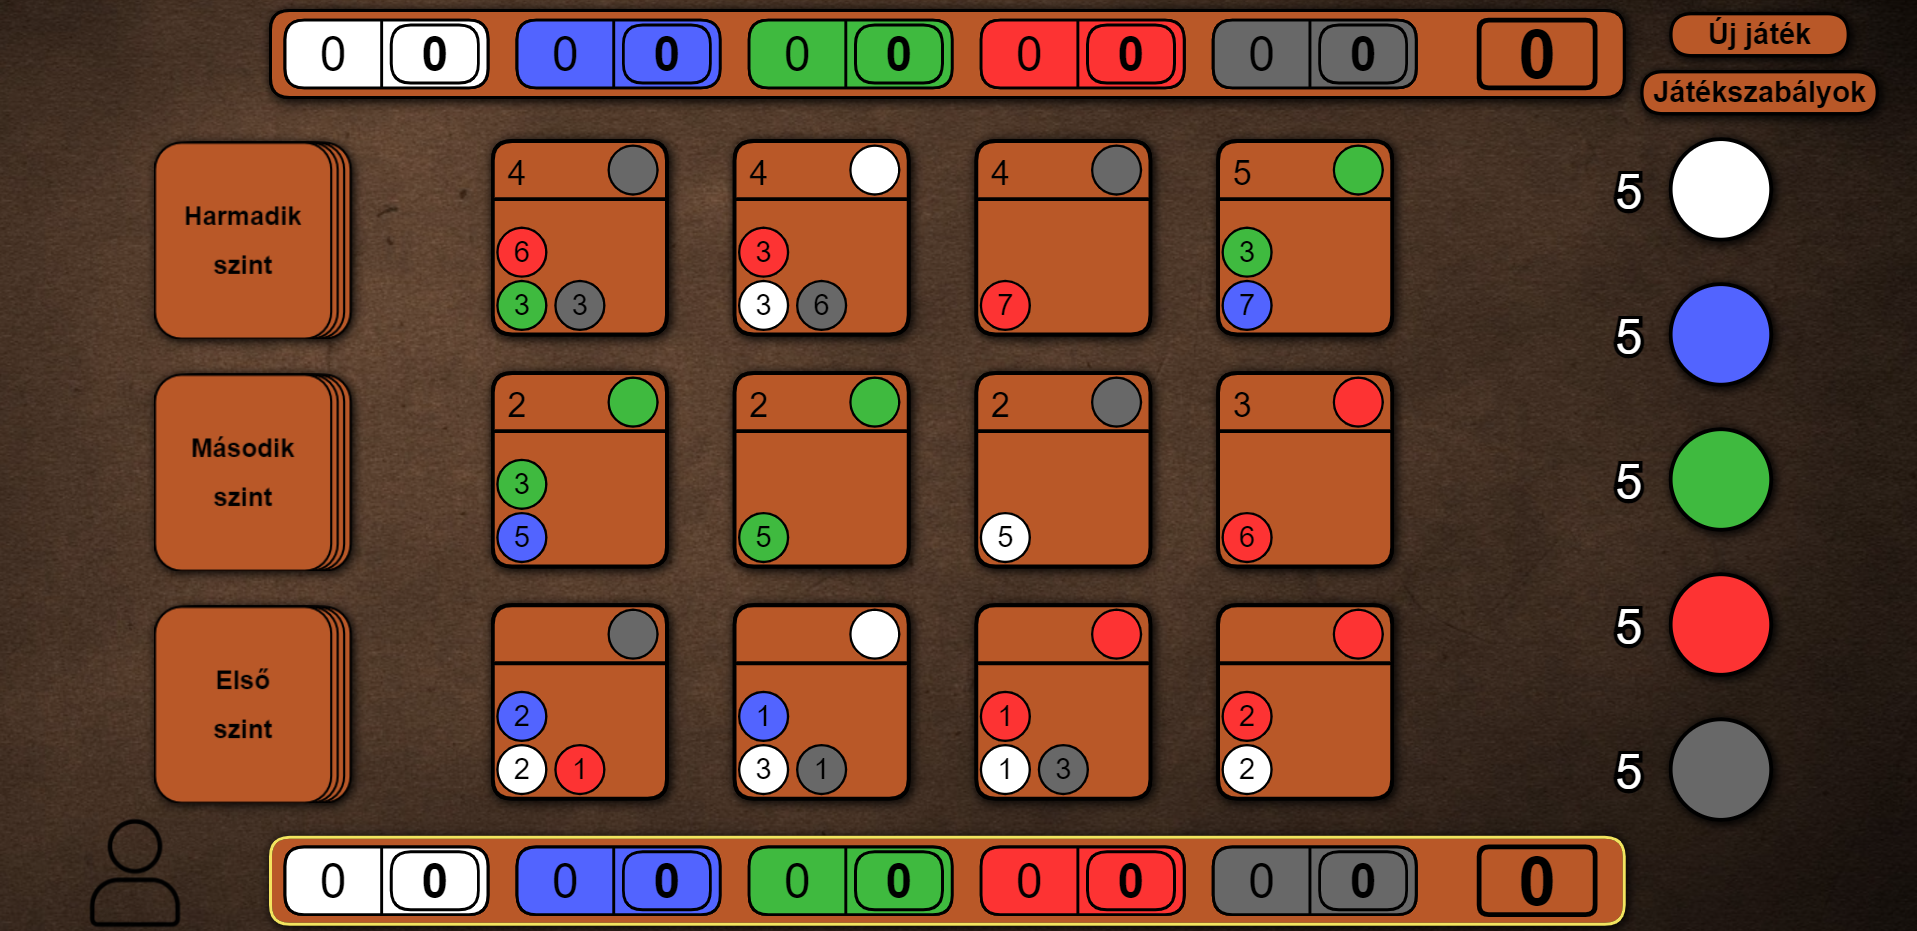
\includegraphics[scale=0.3]{images/screen_structure.png}
\caption{A játék végleges kinézete.}
\label{fig:screen_structure}
\end{figure}


\Section{A játék működése}

Az általam leszűkített szabályrendszer alapú játék megvalósításához a JavaScriptet, a megjelenítéséhez pedig főleg a HTML5 Canvast, minimálisan pedig a CSS-t használtam. A projekt kezdetekor a kártyák megjelenítésével foglalkoztam. Megvalósítottam a kártyák megjelenítését, külső fájlból való betöltését, és az ezáltal kapott adatok alapján a tulajdonságaik elhelyezését is.













%Nyers adatok, parancssori kimenetek megjelenítéséhez a \texttt{verbatim} környezetet lehet használni.
%begin{verbatim}
% some commands with arguments
% 2 3 4 5
% _
%end{verbatim}
